
\section{\sys Design}
\subsection{\sys and Curetprobe}\label{sec:curetprobe}
\xiangyu{Is this name for the subsection better? From \sys{} to Curetprobe}

\noindent Cuprobe provides eBPF-style uprobe/uretprobe hooks for GPU functions at user level. The example below traces a tiled matrix multiply (\texttt{matMulTiled}), counting calls and measuring total time with standard eBPF maps:

\begin{minted}[highlightlines=false,fontsize=\small]{c}
SEC("cuprobe/_Z11matMulTiledPKfS0_Pf")
int cuprobe_matMulTiled(struct pt_regs *ctx) {
    u32 pid = bpf_get_current_pid_tgid() >> 32;
    u64 ts  = bpf_ktime_get_ns();
    bpf_map_update_elem(&start_ts, &pid, &ts, BPF_ANY);
    u64 one = 1, *cnt = bpf_map_lookup_elem(&call_count,
        &pid);  // increment call count
    if (cnt) *cnt += 1;
    else    bpf_map_update_elem(&call_count, &pid, &one,
        BPF_ANY);
}
SEC("curetprobe/_Z11matMulTiledPKfS0_Pf")
int curetprobe_matMulTiled(struct pt_regs *ctx) {
    u32 pid = bpf_get_current_pid_tgid() >> 32;
    u64 *tsp = bpf_map_lookup_elem(&start_ts, &pid);
    if (!tsp) return 0;
    u64 delta = bpf_ktime_get_ns() - *tsp;
    bpf_map_delete_elem(&start_ts, &pid);
    u64 *total = bpf_map_lookup_elem(&total_time_ns,
            &pid); // accumulate execution time
    if (total) {
        *total += delta;
        bpf_map_update_elem(&total_time_ns, &pid,
            total, BPF_EXIST);
    } else {
        bpf_map_update_elem(&total_time_ns, &pid,
            &delta, BPF_NOEXIST);
    }
}
\end{minted}

\noindent Curetprobe lifts the same semantics onto the device by JIT–translating probe handlers into PTX and injecting them into running kernels. Entry/exit trampolines record per‐warp timestamps and update shared eBPF maps, preserving map semantics and enabling function-level profiling without kernel reloads.

\subsection{Userspace eBPF integration}
\begin{figure}
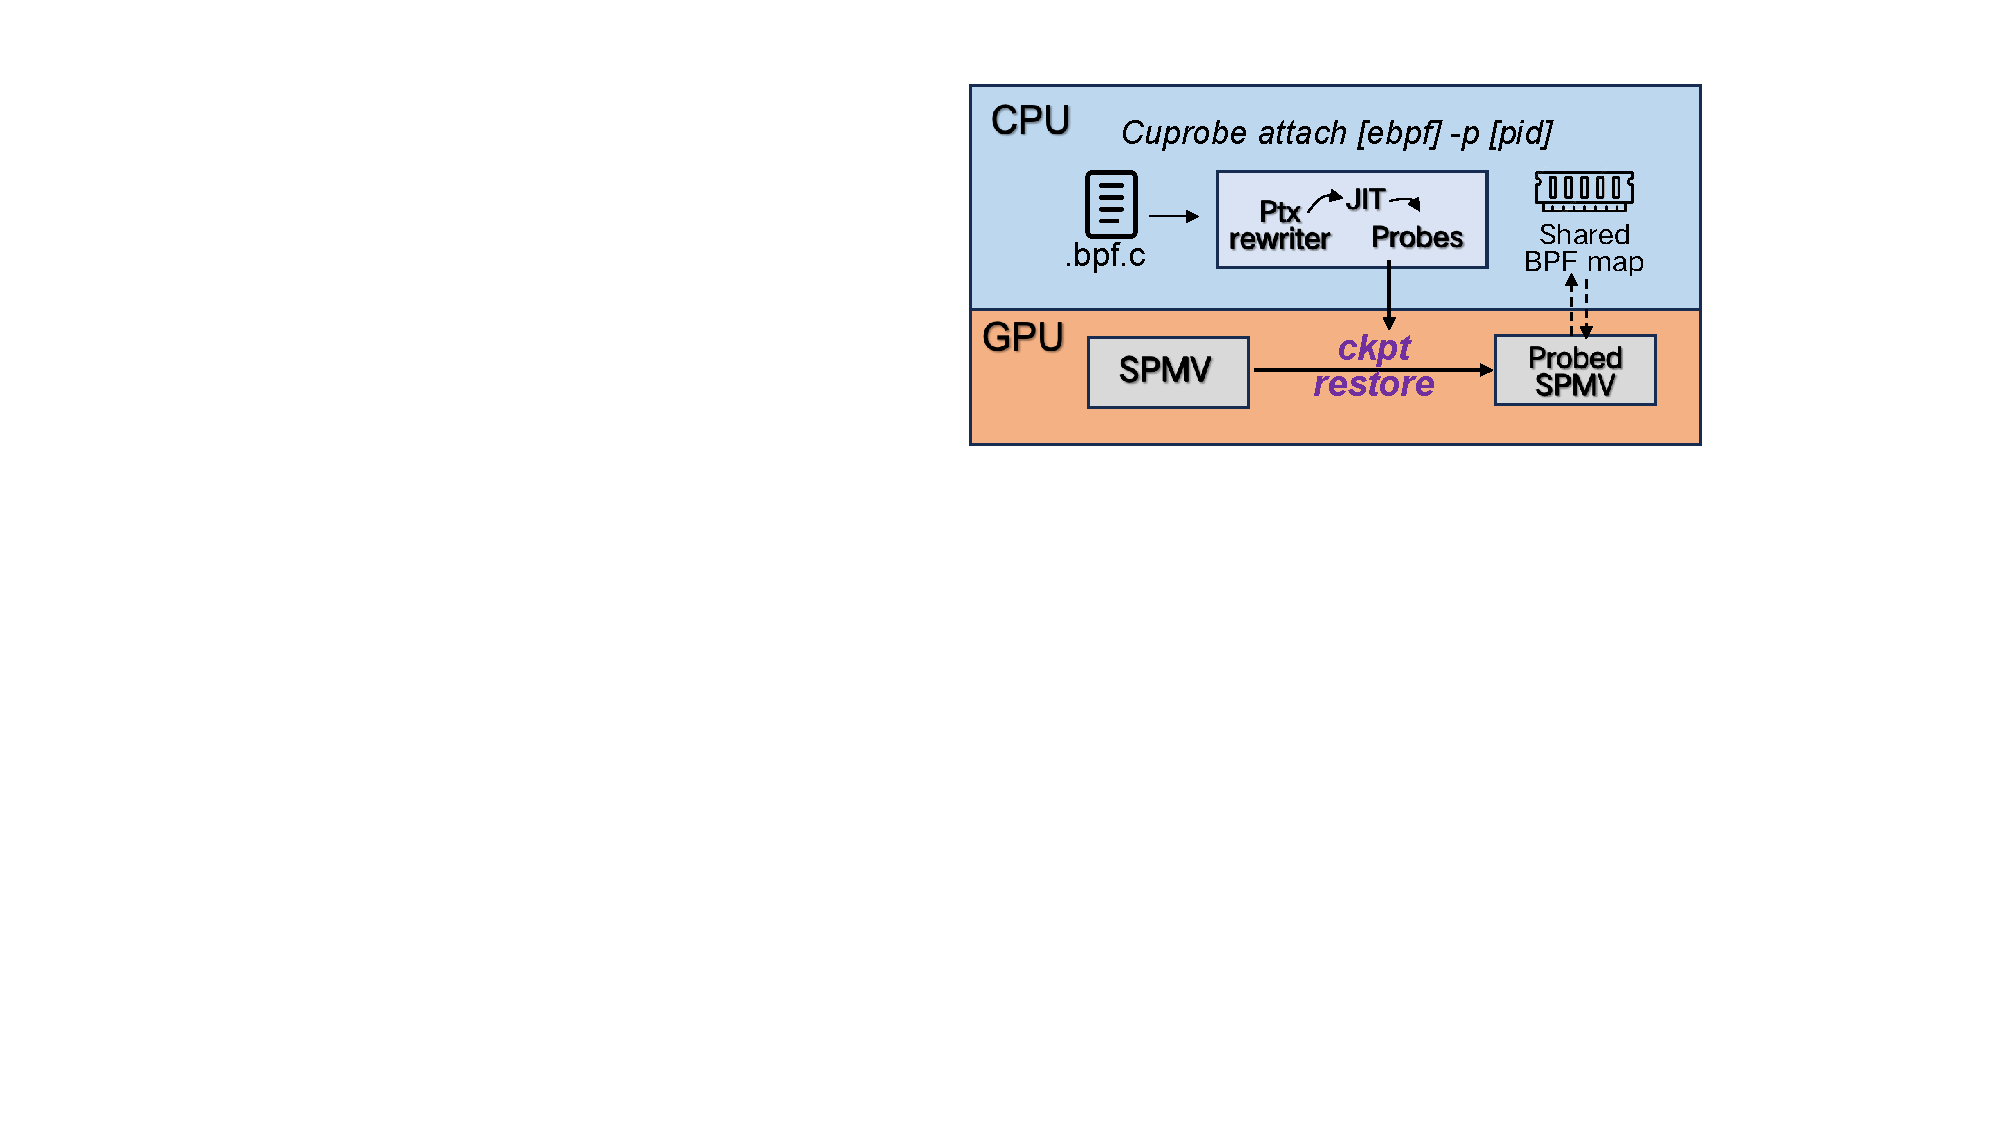
\includegraphics[width=0.8\columnwidth]{img/main.pdf}
\vspace{-.5ex}
\caption{\sys Design}
\label{fig:system-design}
\end{figure}

Figure~\ref{fig:system-design} shows a unified user-space eBPF runtime that keeps verification, JIT, and maps in user space by default. \xiangyu{Source eBPF programs are compiled to standard bytecode} using \xiangyu{existing} tools such as \texttt{clang}, \texttt{bpftool}, or \texttt{bpftrace}. Programs compiled with \texttt{clang}/\texttt{libbpf} write to maps in a shared-memory region (e.g., \texttt{boost::managed\_shared\_memory}) visible to CPU threads and GPU kernels. \xiangyu{Instead of} loading directly into the kernel, this bytecode is handed off to a user‐space runtime (e.g., via \texttt{libbpf}) that includes a user‐space verifier and JIT compiler (\texttt{bpftime‐syscall.so}), enabling safety checks and transformations without requiring elevated privileges. On demand, eBPF bytecode is translated to PTX and injected at GPU hook points so device-side probes write into the same maps, yielding real-time, low-overhead cross CPU–GPU observability.

\begin{figure}[ht]
  \centering
  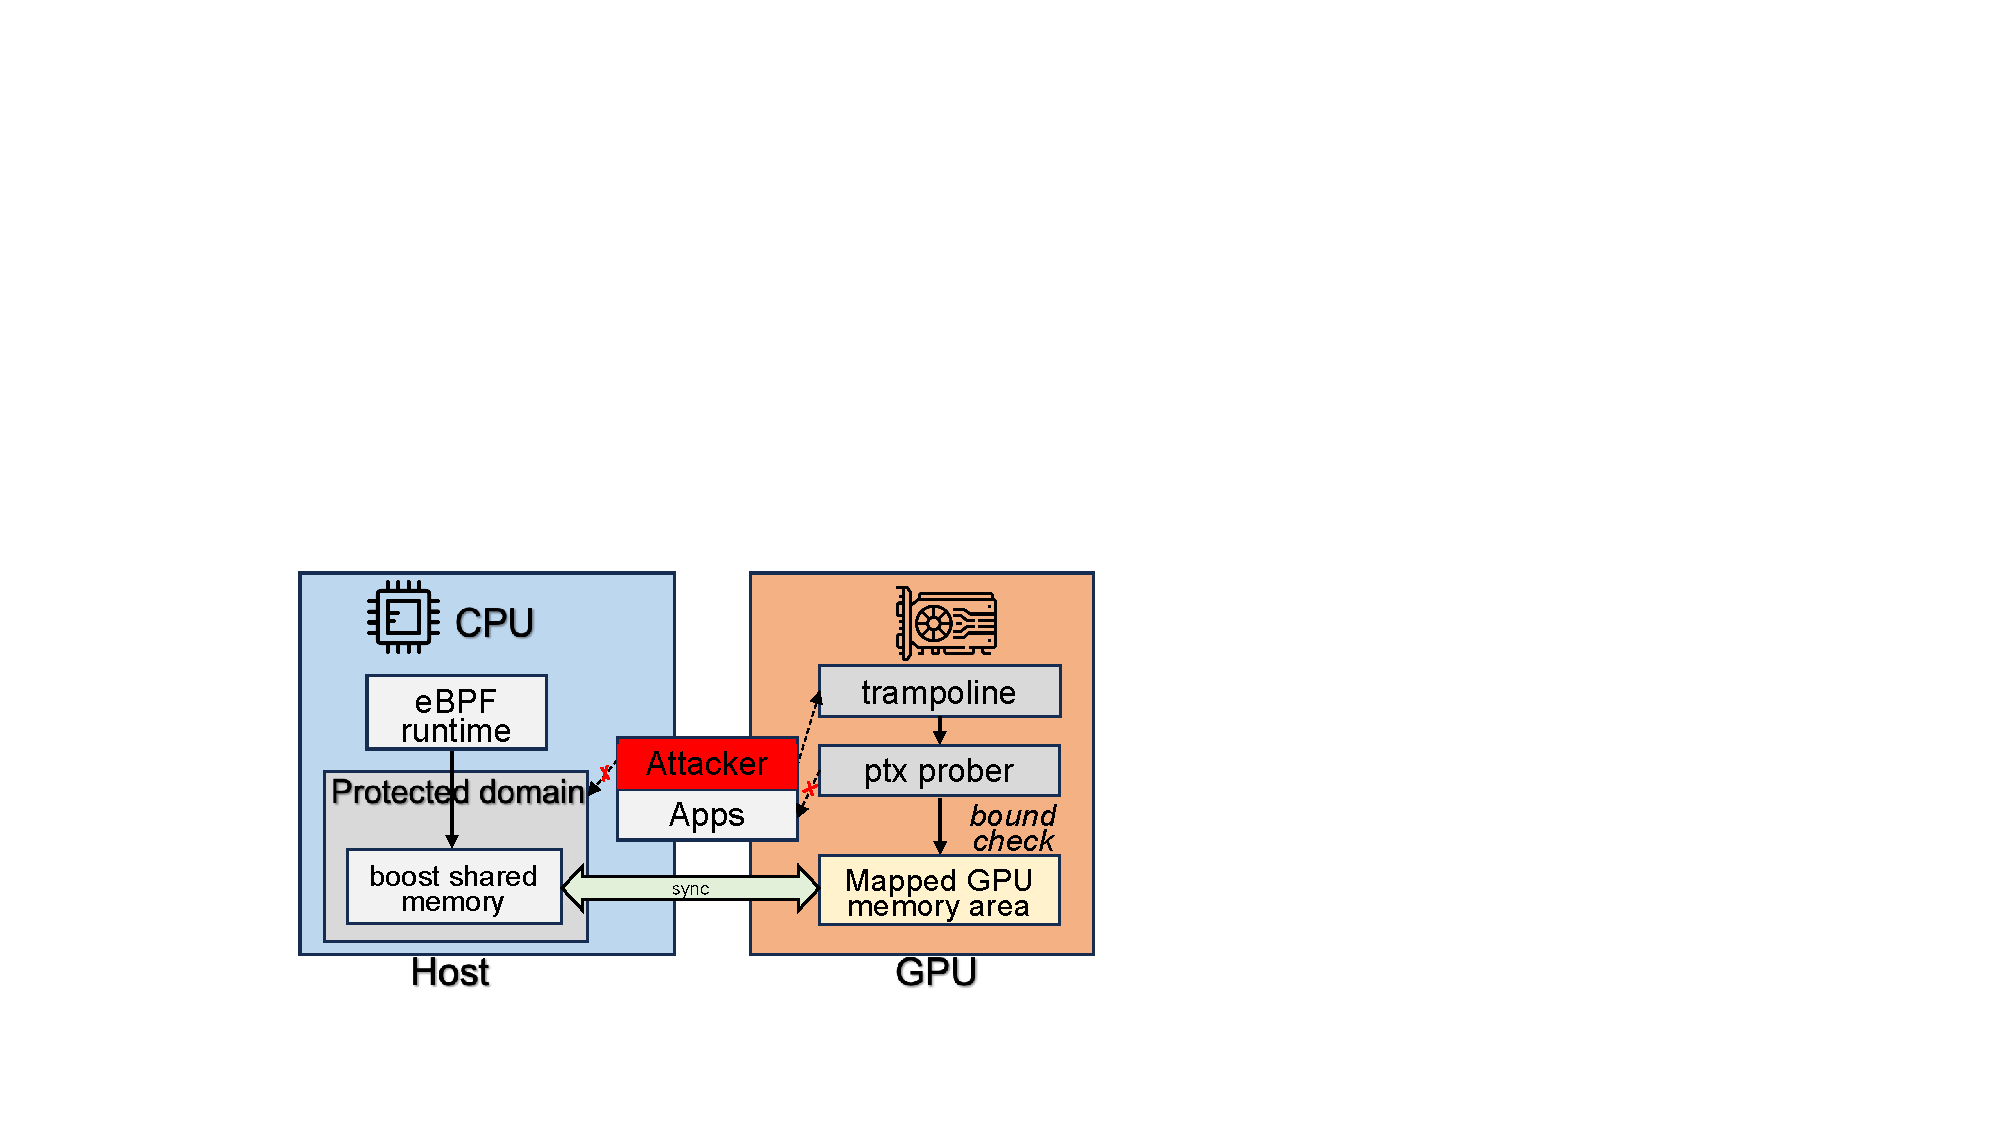
\includegraphics[width=.82\linewidth]{img/gate.pdf}
  \vspace{-.5ex}
  \caption{\sys Gate design for CPU–GPU communication, showing the MPK+CFI‐protected shared memory region, trampoline hooks, and PTX injector within the isolation boundary.}
  \label{fig:mpk_gate}
\end{figure}
\subsection{\sys Gate}

\Cref{fig:mpk_gate} summarizes isolation and coordination. The runtime runs in an MPK/CFI-protected domain and mediates all updates to a shared region mapped by CPU and GPU. A persistent kernel jumps via trampolines into a PTX injector to execute the latest snippet from shared memory, then resumes. Static bound checks prevent access outside the protected region, enabling safe, live instrumentation.

\subsection{GPU Trampoline}\label{sec:gpu_trampoline}

To instrument long-running kernels in place, \sys{} uses tiny PTX trampolines at entry/exit or hot sites. When reached, execution briefly diverts to our snippet and then resumes. Each trampoline:
\begin{itemize}[leftmargin=*,itemsep=0pt]
  \item \textbf{Save:} store minimal live state to a per‐warp scratch buffer.
  \item \textbf{Probe:} jump to the injected PTX (from eBPF) to read/update maps or record events.
  \item \textbf{Restore:} reload state and resume the original control flow.
\end{itemize}
Trampolines are patched atomically at JIT time and confined to the protected domain (\S\ref{sec:isolation}); we observe sub–\(1\,\mu\)s overhead per invocation in practice.


\section{\sys{} Implementation}
In this section, we will talk about the \sys implementation.\xiangyu{Suggest removing this sentence.}
\label{sec:design}

% [Removed: Self‐Modifying Code / POS / checkpoint & restore / record & replay]

\subsection{Shared Memory}

We place maps and coordination buffers in \texttt{managed\_shared\_memory} for zero-copy CPU/GPU access, reducing marshaling and latency. Coherent platforms (e.g., Grace Hopper) further scale capacity and minimize synchronization costs via fabric-managed coherence. Emerging architectures such as NVIDIA's Grace Hopper \xiangyu{promise --> offers} hardware‐coherent, large‐scale memory pools over high‐speed interconnects.


\subsection{Cross‐Domain Memory Synchronization}

On non-coherent systems, cross-domain visibility requires explicit barriers (device \_\_threadfence\_system and host stream sync). \xiangyu{The reason is that }to transfer writes from the GPU to the CPU, the device must execute \_\_threadfence\_system() to flush any outstanding writes into system‐visible memory, followed by a host-side cudaStreamSynchronize() to wait for the GPU to complete. We encapsulate these as a simple device/host pair to centralize tuning and reduce boilerplate:
\begin{minted}[highlightlines=false,fontsize=\small]{c}
// Ensure GPU writes become visible to the CPU
__device__ inline void memsys_bar_gpu() {
    __threadfence_system();
}
// Wait for the GPU on the given stream
static inline void memsys_bar_cpu(cudaStream_t stream =
        0) {
    cudaStreamSynchronize(stream);
}
\end{minted}
In a persistent kernel, call the GPU fence before reading shared state; after host updates, synchronize the stream to ensure visibility. This two-call barrier hides cross-domain complexity. On the host side, memsys\_bar\_cpu() calls cudaStreamSynchronize() on a specified stream to wait for the GPU to finish its pending commands, including memory writes. This wrapper simplifies code, clarifies intent, and centralizes performance tuning. \xiangyu{I have one suggestion. If we have supporting results for these statements in the eval section, we should point them to relevant sections}
\begin{minted}[highlightlines=false,fontsize=\small]{c}
using namespace boost::interprocess;
__device__ int *shared_flag;
__global__ void persistent_kernel() {
    memsys_bar_gpu();// Ensure CPU writes are visible
    int cmd = *shared_flag;
    // Jump into PTX injector...
}
int main() {
    managed_shared_memory shm(open_or_create, "MyShm"
        , 1 << 20);
    int *flag = shm.construct<int>("Flag")(0)[1];
    *flag = 42;              // Write command
    memsys_bar_cpu(0);       // Ensure GPU sees update
    persistent_kernel<<<grid, block>>>();
    cudaDeviceSynchronize();
}
\end{minted}
Looking into systems like NVIDIA's Grace Hopper, which support hardware cache coherence across CPU and GPU, these explicit barriers will become unnecessary. Under a coherent interconnect such as NVLink/CXL, cache lines are automatically propagated and merged at the L2/L3 levels, eliminating the need for manual \_\_threadfence\_system() or stream synchronizations. Early measurements indicate that cross-domain latency on such platforms can shrink from tens of microseconds to just hundreds of nanoseconds, reducing synchronization overhead by an order of magnitude and enabling truly low-latency shared-memory coordination.

\subsection{Synchronization}
We use host atomics/interprocess primitives and device CUDA atomics/fences over well-defined layouts in shared memory. To reduce contention, only a subset of threads performs atomics while others proceed in parallel.

\subsection{PTX Generation \& Injection}\label{sec:ptx_injection}

User/eBPF logic triggers JIT generation of PTX snippets that are installed via in-place patching ("PTX injection"). Snippets interoperate with eBPF maps and shared buffers to support flexible, low-latency instrumentation without relaunching kernels.

\paragraph{Trampoline Mechanism}
At runtime we patch candidate sites (entry, memory access, barriers) with a tiny PTX stub that:
\begin{itemize}[leftmargin=*,itemsep=0pt]
  \item Saves the minimal GPU register and predicate state.
  \item Jumps into the injected instrumentation snippet.
  \item Restores the original state and resumes normal execution.
\end{itemize}
These trampolines are linked into the device's code image via in-place patching of branch targets, enabling fine-grained hooking without requiring kernel relaunch or full recompilation. Our trampoline generator handles label resolution, register allocation, and insertion of necessary synchronization primitives to avoid hazards.



\subsection{Isolation Requirement}\label{sec:isolation}

Dynamic PTX injection and trampoline-based instrumentation introduce new code into live GPU kernels, which \xiangyu{must be prevented from --> might bring the risk of} corrupting application state or violating memory safety. \sys therefore runs injected snippets in a protected domain.

\paragraph{Guardian-inspired GPU Partition}
Drawing on Guardian~\cite{pavlidakis2024guardian}, \sys partitions GPU address space at runtime and fences every load/store with lightweight masking:

\begin{itemize}[leftmargin=*,itemsep=0pt]
  \item \textbf{Dynamic Partitioning:} At initialization, \sys{} uses one partition of entire GPU memory. Each instrumentation snippet is tagged with its owner's partition ID.
  \item \textbf{PTX-Level Bounds Fencing:} Before every memory access, bitwise AND/OR operations mask the computed address into the tenant's partition range, guaranteeing that out-of-bounds addresses wrap harmlessly within the correct domain.
  \item \textbf{Client–Server Enforcement:} Inspired by Guardian's client–server model, all CUDA calls (allocations, copies, launches) are intercepted and forwarded to a trusted Manager. This server maintains the partition bounds table and rejects any operation that would violate domain isolation.
\end{itemize}

\paragraph{Runtime Sandbox Integration}
During JIT compilation, \sys{} wraps each PTX snippet in a minimal prologue/epilogue sequence that:
%\begin{itemize}[leftmargin=*,itemsep=0pt]
  %\item
  a) Saves a live register state to a safe context.
  %\item
  b) Applies bitwise partition masking and invokes the instrumentation logic.
  %\item
  c) Restores registers and resumes normal kernel execution.
%\end{itemize}

Combining Guardian-style fencing with trampolines and shared-memory coordination ensures injected code remains isolated from application kernels.
